\documentclass[titlepage, twocolumn]{article}

\usepackage{graphicx}
\graphicspath{{./figures}}

\title{%
    Engineering Physics 353 Final Report \\
    \large Team 14 - ``Team 4"}
\author{Nathan Van Rumpt, Eric Souder}
\date{April 2023}

\begin{document}
\maketitle

\begin{abstract}
    This is the abstract.
\end{abstract}

\section{Background}

\section{Overall Architecture}

\section{Navigation}
    Robot navigation was accomplished with an almost entirely classical control system, using minimal neural network-based approaches and instead using manually-tuned computer vision and classical control techniques. 

    The navigation controller was composed of two ROS nodes: The `State Machine' node was composed of a finite state machine and the `Navigate' node contained a set of navigation algorithms for different scenarios, selecting an appropriate algorithm based on the state reported by the state machine. States were communicated internally between the two nodes via a ROS topic.
    
    \subsection{State Machine}
        The finite state machine responsible for controlling the robot's navigation state was composed primarily of a number of state classes, representing a unique navigational state and a state machine class responsible for orchestrating the transitions between them. Each state class, such as the `Pave Navigate' or `Junction Wait' states, is a subclass of an abstract parent class which defines an `evaluate transition' interface which determines the next state to enter and either returns itself to remain in the current state or generates a new state object to transition into. The state machine class calls this method each frame to determine which state the robot should be in, and then broadcasts that state to the navigation node via a ROS topic. The overall state machine diagram is shown in Figure~\ref{fig:statemachine}.

        \begin{figure}
            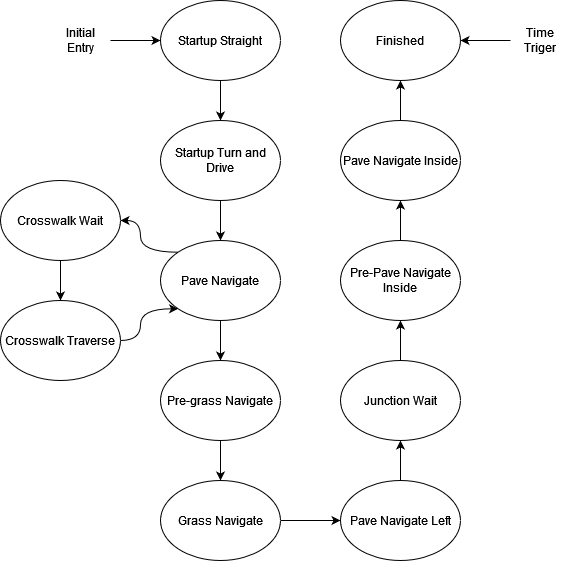
\includegraphics[width=\linewidth]{statemachine.png}
            \caption{Diagram of the robot state machine.}
            \label{fig:statemachine}
        \end{figure}

        As behaviors such as waiting at the crosswalk or waiting for the truck are defined as discrete states, the crosswalk and pedestrian detection as well as junction and truck detection are part of the state transition logic contained in certain `evaluate transition' methods.

        \subsubsection{Crosswalk Pedestrian Detection}
            When navigating over the first section of paved track, two crosswalks with pedestrians must be safely crossed without hitting any pedestrians. Detection of both crosswalks and pedestrians is performed by methods within the `PedestrianDetector' class. First, crosswalks were detected using simple HSV colour thresholding. [figure here]. A crosswalk was considered 'detected' when 1500 total pixels matching the range of colours associated with the red crosswalk stop line were detected in the bottom 100 rows of the image. Although 1500 pixels is less than 2 full horizontal rows - much less than the size of the detection area - the need for a large area was the result of the relative high velocity which meant that the robot may only receive one or two frames to detect the crosswalk, so the larger area was chosen as a compromise between guaranteeing detection of the stop line and constantly stopping at around the same location. It also provides detection capability if the line is approached at an angle. This hedges against a possible 10 point loss from hitting a pedestrian of other parts of the navigation system fail.

            Pedestrians were detected using HSV thresholding to detect their blue jeans, similarly to the crosswalk detection. [figure here]. However, since the location (not just boolean presence) of the pedestrians was needed, erosion and dilation were used to merge the thresholded areas together into fewer, larger `blobs'. The algorithm then finds the contours of each `blob' and selects the largest as the most likely choice to be the pedestrian. Each frame, A bounding box is drawn around it, and its position is found.

            As a result of the repeatability of our pavement navigation algorithms, the edges of the crosswalk were able to be hard-coded into the pedestrian detector. The state machine tracks the position of the detector, and waits for it to be found in the crossawlk and then to exit the crosswalk. At this point, we can gurantee the maximum amount of time that the pedestrian will not be in the crosswalk, adnd the state machine is then able to transition to a `Crosswalk Traverse' sprint across the crosswalk before resuming normal pavement navigation. 
            
        \subsection{Junction and Truck Detection}
            
    \subsection{Navigation Algorithms}
    \subsection{Performance}

\section{License Plate Detection}

\section{Conclusion}

\end{document}